\documentclass[tikz, margin=2]{standalone}
\usepackage{amsmath}


% Commands for colors
\newcommand{\B}{black}
\newcommand{\W}{white}
% Command to draw a necklace
\newcommand{\drawNecklace}[6]{
    \draw (#1,#2) circle (1);
    \filldraw[fill=#3] (#1,#2+1) circle (.2);
    \filldraw[fill=#4] (#1+1,#2) circle (.2);
    \filldraw[fill=#5] (#1,#2-1) circle (.2);
    \filldraw[fill=#6] (#1-1,#2) circle (.2);
}


\begin{document}
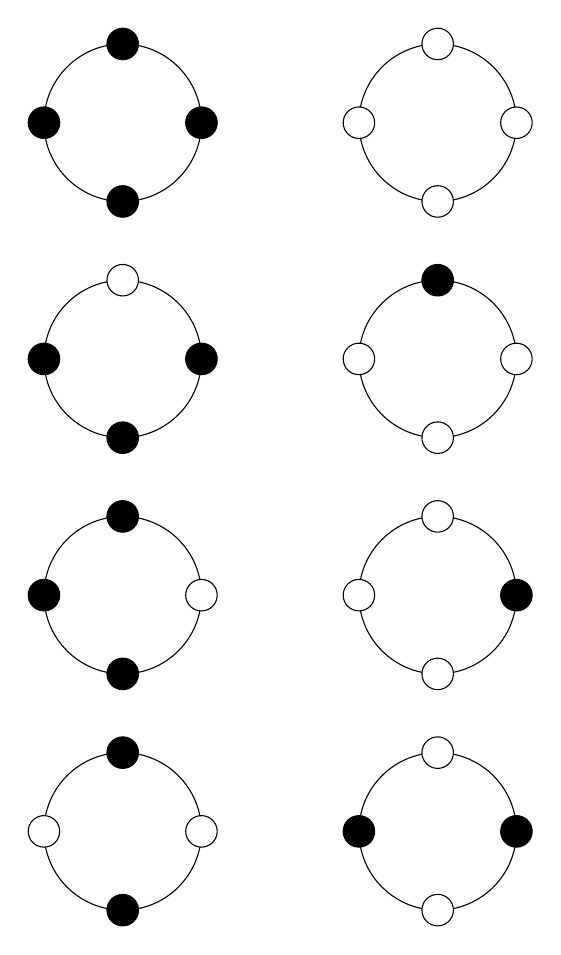
\begin{tikzpicture}

% All black and all white colorings
\drawNecklace{-2}{0}{\B}{\B}{\B}{\B}
\drawNecklace{ 2}{0}{\W}{\W}{\W}{\W}

% One black or one white
\drawNecklace{-2}{-3}{\W}{\B}{\B}{\B}
\drawNecklace{ 2}{-3}{\B}{\W}{\W}{\W}
\drawNecklace{-2}{-6}{\B}{\W}{\B}{\B}
\drawNecklace{ 2}{-6}{\W}{\B}{\W}{\W}

% Two of each
\drawNecklace{-2}{-9}{\B}{\W}{\B}{\W}
\drawNecklace{ 2}{-9}{\W}{\B}{\W}{\B}

\end{tikzpicture}
\end{document}
